% Options for packages loaded elsewhere
\PassOptionsToPackage{unicode}{hyperref}
\PassOptionsToPackage{hyphens}{url}
\PassOptionsToPackage{dvipsnames,svgnames,x11names}{xcolor}
%
\documentclass[
]{article}
\title{Supplementary Material 1: Bluegill Growth Card Data Cleaning and
Aggregation}
\author{}
\date{\vspace{-2.5em}}

\usepackage{amsmath,amssymb}
\usepackage{lmodern}
\usepackage{iftex}
\ifPDFTeX
  \usepackage[T1]{fontenc}
  \usepackage[utf8]{inputenc}
  \usepackage{textcomp} % provide euro and other symbols
\else % if luatex or xetex
  \usepackage{unicode-math}
  \defaultfontfeatures{Scale=MatchLowercase}
  \defaultfontfeatures[\rmfamily]{Ligatures=TeX,Scale=1}
\fi
% Use upquote if available, for straight quotes in verbatim environments
\IfFileExists{upquote.sty}{\usepackage{upquote}}{}
\IfFileExists{microtype.sty}{% use microtype if available
  \usepackage[]{microtype}
  \UseMicrotypeSet[protrusion]{basicmath} % disable protrusion for tt fonts
}{}
\makeatletter
\@ifundefined{KOMAClassName}{% if non-KOMA class
  \IfFileExists{parskip.sty}{%
    \usepackage{parskip}
  }{% else
    \setlength{\parindent}{0pt}
    \setlength{\parskip}{6pt plus 2pt minus 1pt}}
}{% if KOMA class
  \KOMAoptions{parskip=half}}
\makeatother
\usepackage{xcolor}
\IfFileExists{xurl.sty}{\usepackage{xurl}}{} % add URL line breaks if available
\IfFileExists{bookmark.sty}{\usepackage{bookmark}}{\usepackage{hyperref}}
\hypersetup{
  pdftitle={Supplementary Material 1: Bluegill Growth Card Data Cleaning and Aggregation},
  colorlinks=true,
  linkcolor={Maroon},
  filecolor={Maroon},
  citecolor={Blue},
  urlcolor={blue},
  pdfcreator={LaTeX via pandoc}}
\urlstyle{same} % disable monospaced font for URLs
\usepackage[margin=1in]{geometry}
\usepackage{color}
\usepackage{fancyvrb}
\newcommand{\VerbBar}{|}
\newcommand{\VERB}{\Verb[commandchars=\\\{\}]}
\DefineVerbatimEnvironment{Highlighting}{Verbatim}{commandchars=\\\{\}}
% Add ',fontsize=\small' for more characters per line
\usepackage{framed}
\definecolor{shadecolor}{RGB}{248,248,248}
\newenvironment{Shaded}{\begin{snugshade}}{\end{snugshade}}
\newcommand{\AlertTok}[1]{\textcolor[rgb]{0.94,0.16,0.16}{#1}}
\newcommand{\AnnotationTok}[1]{\textcolor[rgb]{0.56,0.35,0.01}{\textbf{\textit{#1}}}}
\newcommand{\AttributeTok}[1]{\textcolor[rgb]{0.77,0.63,0.00}{#1}}
\newcommand{\BaseNTok}[1]{\textcolor[rgb]{0.00,0.00,0.81}{#1}}
\newcommand{\BuiltInTok}[1]{#1}
\newcommand{\CharTok}[1]{\textcolor[rgb]{0.31,0.60,0.02}{#1}}
\newcommand{\CommentTok}[1]{\textcolor[rgb]{0.56,0.35,0.01}{\textit{#1}}}
\newcommand{\CommentVarTok}[1]{\textcolor[rgb]{0.56,0.35,0.01}{\textbf{\textit{#1}}}}
\newcommand{\ConstantTok}[1]{\textcolor[rgb]{0.00,0.00,0.00}{#1}}
\newcommand{\ControlFlowTok}[1]{\textcolor[rgb]{0.13,0.29,0.53}{\textbf{#1}}}
\newcommand{\DataTypeTok}[1]{\textcolor[rgb]{0.13,0.29,0.53}{#1}}
\newcommand{\DecValTok}[1]{\textcolor[rgb]{0.00,0.00,0.81}{#1}}
\newcommand{\DocumentationTok}[1]{\textcolor[rgb]{0.56,0.35,0.01}{\textbf{\textit{#1}}}}
\newcommand{\ErrorTok}[1]{\textcolor[rgb]{0.64,0.00,0.00}{\textbf{#1}}}
\newcommand{\ExtensionTok}[1]{#1}
\newcommand{\FloatTok}[1]{\textcolor[rgb]{0.00,0.00,0.81}{#1}}
\newcommand{\FunctionTok}[1]{\textcolor[rgb]{0.00,0.00,0.00}{#1}}
\newcommand{\ImportTok}[1]{#1}
\newcommand{\InformationTok}[1]{\textcolor[rgb]{0.56,0.35,0.01}{\textbf{\textit{#1}}}}
\newcommand{\KeywordTok}[1]{\textcolor[rgb]{0.13,0.29,0.53}{\textbf{#1}}}
\newcommand{\NormalTok}[1]{#1}
\newcommand{\OperatorTok}[1]{\textcolor[rgb]{0.81,0.36,0.00}{\textbf{#1}}}
\newcommand{\OtherTok}[1]{\textcolor[rgb]{0.56,0.35,0.01}{#1}}
\newcommand{\PreprocessorTok}[1]{\textcolor[rgb]{0.56,0.35,0.01}{\textit{#1}}}
\newcommand{\RegionMarkerTok}[1]{#1}
\newcommand{\SpecialCharTok}[1]{\textcolor[rgb]{0.00,0.00,0.00}{#1}}
\newcommand{\SpecialStringTok}[1]{\textcolor[rgb]{0.31,0.60,0.02}{#1}}
\newcommand{\StringTok}[1]{\textcolor[rgb]{0.31,0.60,0.02}{#1}}
\newcommand{\VariableTok}[1]{\textcolor[rgb]{0.00,0.00,0.00}{#1}}
\newcommand{\VerbatimStringTok}[1]{\textcolor[rgb]{0.31,0.60,0.02}{#1}}
\newcommand{\WarningTok}[1]{\textcolor[rgb]{0.56,0.35,0.01}{\textbf{\textit{#1}}}}
\usepackage{graphicx}
\makeatletter
\def\maxwidth{\ifdim\Gin@nat@width>\linewidth\linewidth\else\Gin@nat@width\fi}
\def\maxheight{\ifdim\Gin@nat@height>\textheight\textheight\else\Gin@nat@height\fi}
\makeatother
% Scale images if necessary, so that they will not overflow the page
% margins by default, and it is still possible to overwrite the defaults
% using explicit options in \includegraphics[width, height, ...]{}
\setkeys{Gin}{width=\maxwidth,height=\maxheight,keepaspectratio}
% Set default figure placement to htbp
\makeatletter
\def\fps@figure{htbp}
\makeatother
\setlength{\emergencystretch}{3em} % prevent overfull lines
\providecommand{\tightlist}{%
  \setlength{\itemsep}{0pt}\setlength{\parskip}{0pt}}
\setcounter{secnumdepth}{-\maxdimen} % remove section numbering
\ifLuaTeX
  \usepackage{selnolig}  % disable illegal ligatures
\fi

\begin{document}
\maketitle

\textbf{Description:} This tutorial describes the process of cleaning,
aggregating, and standardizing output from Zooniverse transcribed data.
The initial data extraction and reduction process from Zooniverse JSON
data output was first run in Python using the panoptes-aggregation
package, a package specifically made for Zooniverse projects, and is not
included in this tutorial (Figure 1). The resulting csv files from this
process come from two Zooniverse workflows 1) Basic tasks - where
volunteers transcribe geographic location, dates of sampling, and
collectors which are fields common to all data card types and 2) Growth
tasks - where volunteers transcribe the number of fish, range and mean
length of the fish, and fish age from growth cards. We combine several
types of tasks from each of these workflows to produce a complete set of
bluegill data from growth cards (Figure 1).

We first clean each of these tasks separately, then aggregate the
datasets, and join them with the comments from the volunteer
transcribers and the lake names that were matched to a local authority
file (Figure 1). Finally, we standardize and quality check units.

\begin{figure}
\centering
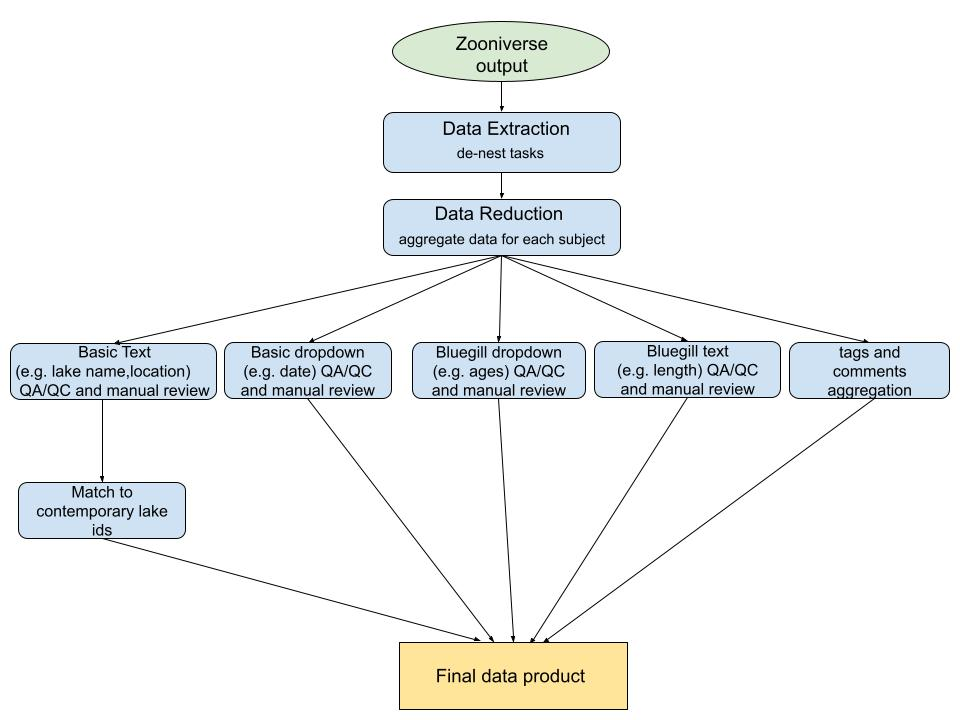
\includegraphics{images/curation_steps.jpg}
\caption{Figure 1: An overview of data curation steps for the Bluegill
growth cards.}
\end{figure}

\begin{center}\rule{0.5\linewidth}{0.5pt}\end{center}

\hypertarget{part-1-load-libraries-and-data}{%
\section{Part 1: Load libraries and
data}\label{part-1-load-libraries-and-data}}

We have several datasets to load that will help us clean and match the
output from Zooniverse. All data sets and code for this tutorial can be
downloaded from github,
\url{https://github.com/CHANGES-UM/data_curation_examples}.

\begin{enumerate}
\def\labelenumi{\arabic{enumi})}
\item
  ``grow\_card\_lake\_match\_13Sep2021.csv'' is a file that links
  historical lakes to the current ``new\_key'', a lake identifier given
  to each lake by the Michigan Department of Natural Resources.
\item
  ``basic\_GROW\_URLs.csv'' is a file that has all of the links to the
  data card images. Take a look at an example image of a data card to
  become familiar with the original data format.
  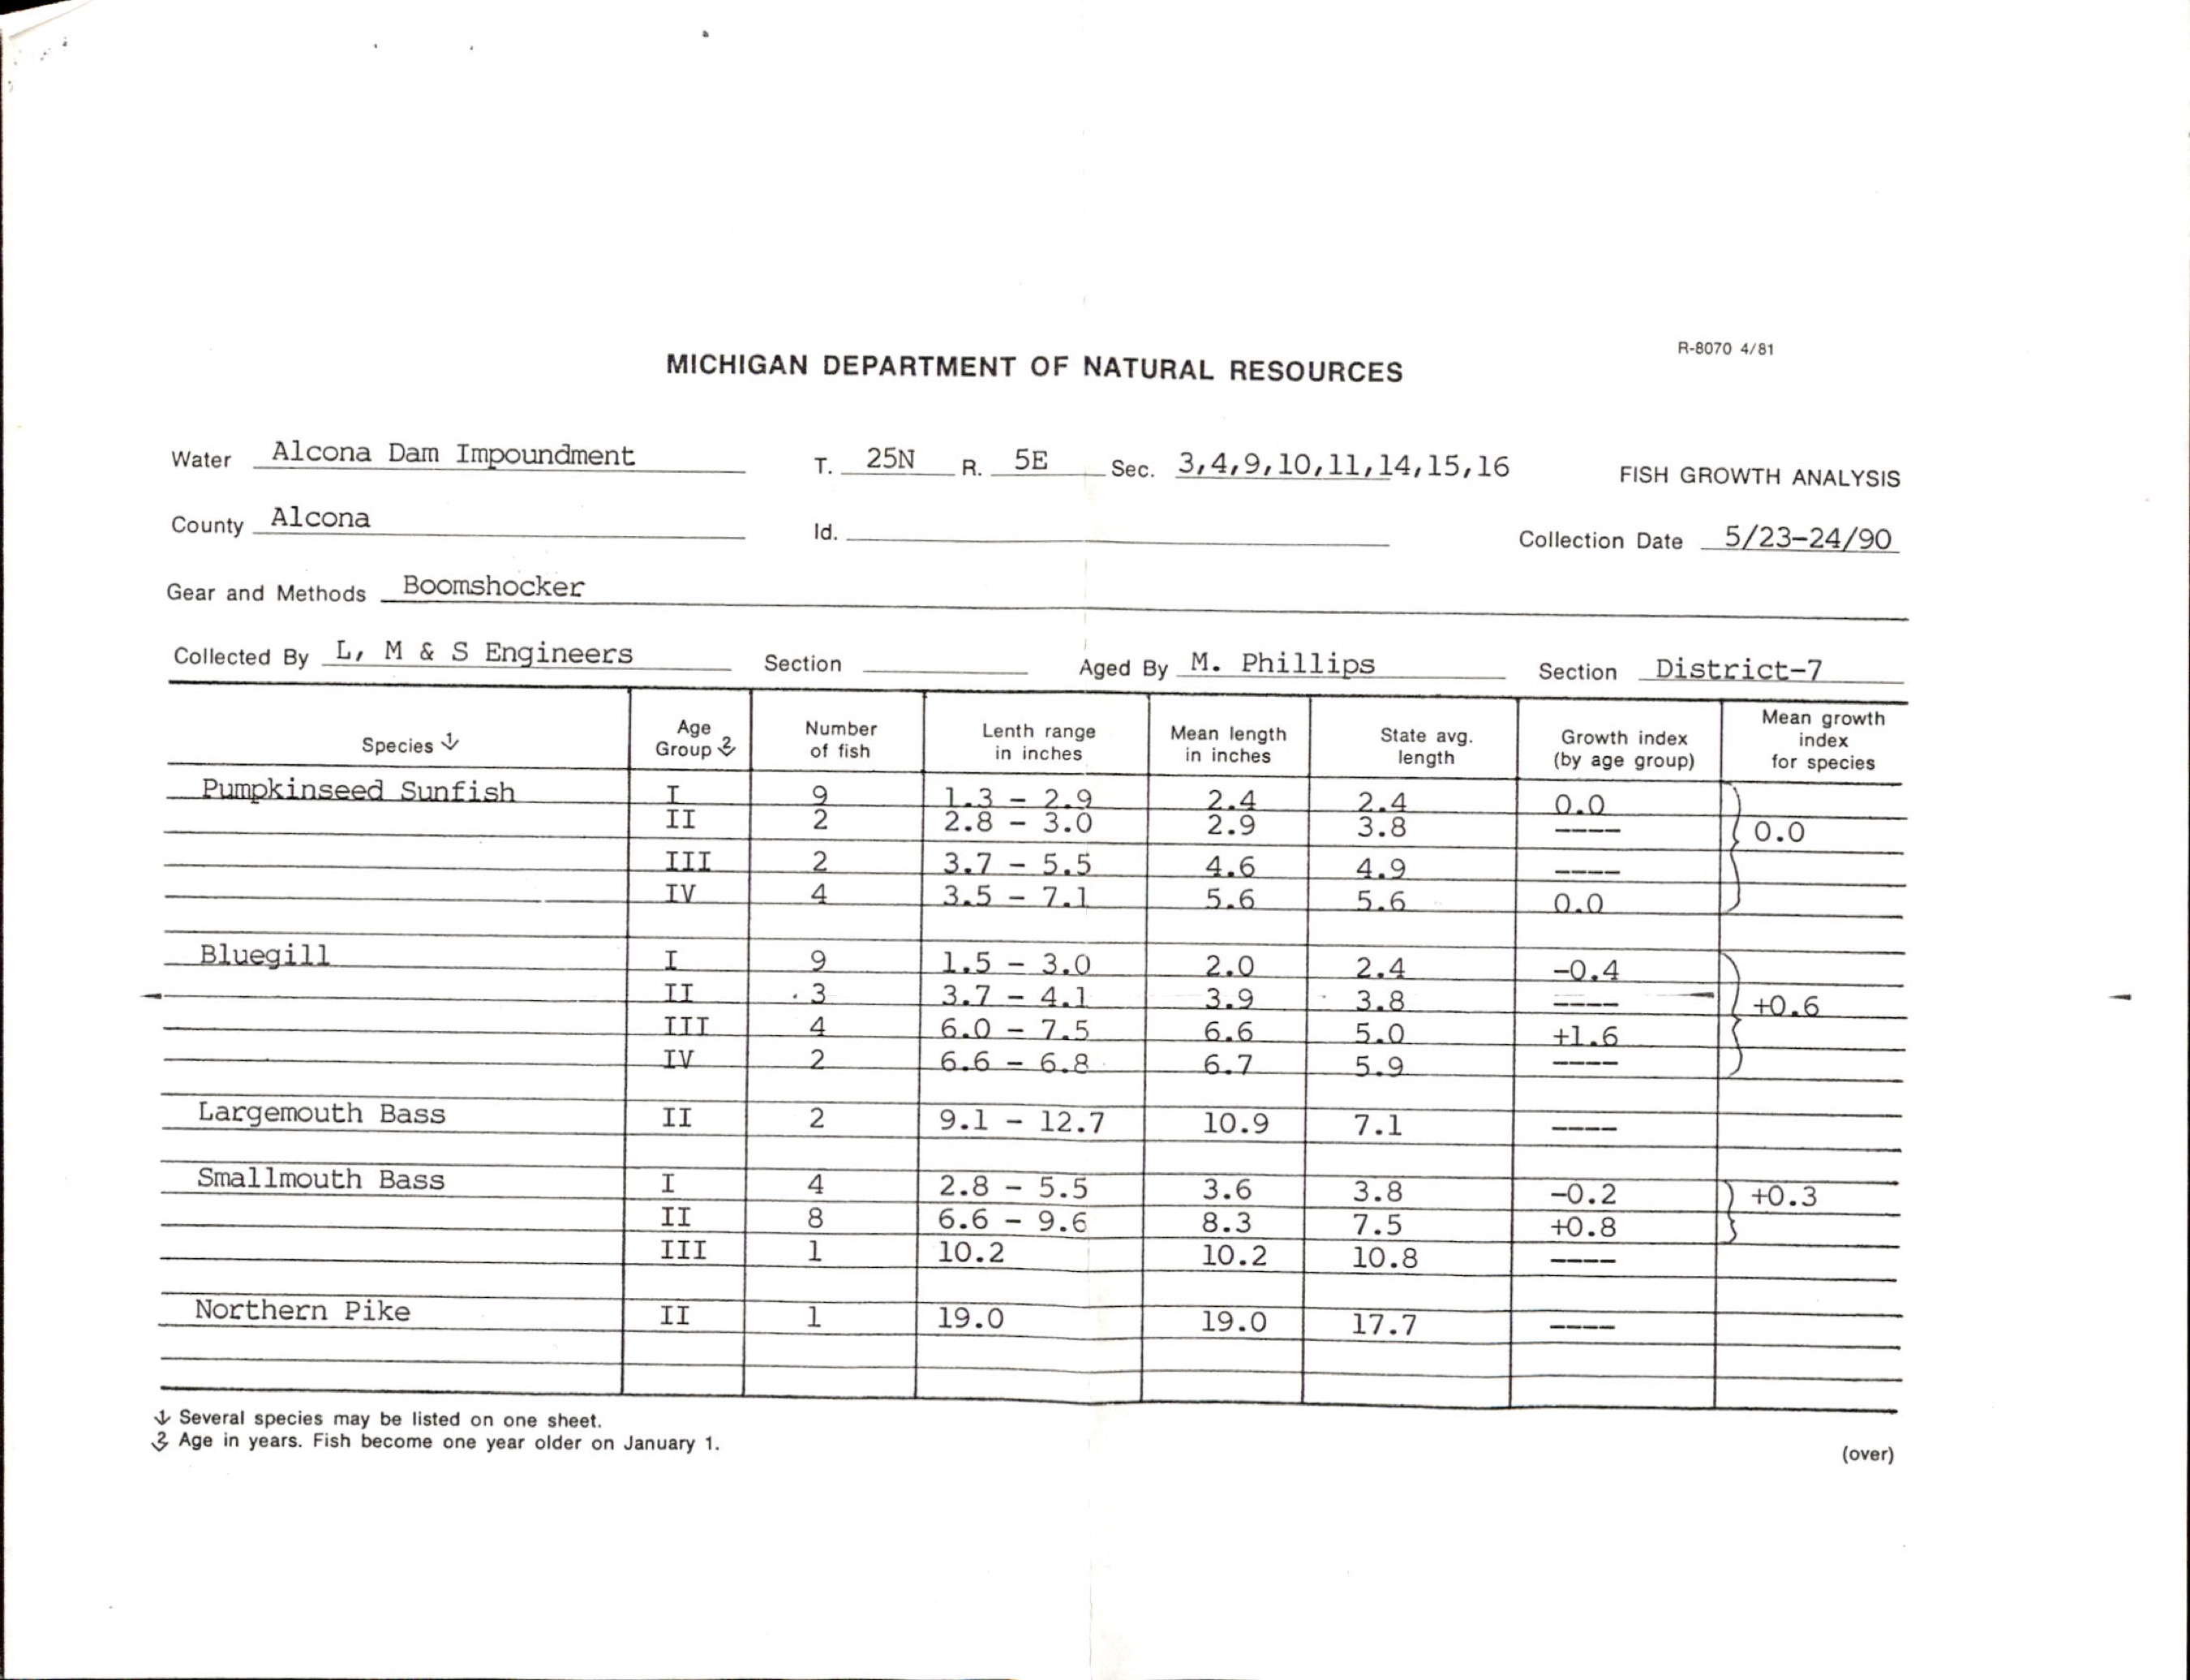
\includegraphics{images/alconadam_grow.jpg}
\item
  ``Basic\_task\_value.csv'' and ``GROW\_task\_values.csv'' are files
  that have the task code from Zooniverse that can be linked to the
  actual task name
\item
  ``Basic\_date\_values.csv'' and ``GROW\_age\_values'' are files that
  have codes from Zooniverse drop down options that link to the actual
  date or the actual age value.
\end{enumerate}

\begin{Shaded}
\begin{Highlighting}[]
\DocumentationTok{\#\#\#\# load libraries \#\#\#\# }
\FunctionTok{library}\NormalTok{(dplyr) }\CommentTok{\# library for data munging }
\FunctionTok{library}\NormalTok{(tidyr) }\CommentTok{\# library for data munging }
\FunctionTok{library}\NormalTok{(stringr) }\CommentTok{\#library for regex functions }
\FunctionTok{library}\NormalTok{(rqdatatable) }\CommentTok{\#join and replace NAs from one table with data from another }

\DocumentationTok{\#\#\#\# load data \#\#\#\# }
\CommentTok{\#read in lake match data where lakes were matched to MDNR authority file   }
\NormalTok{lake\_match }\OtherTok{\textless{}{-}}\FunctionTok{read.csv}\NormalTok{(}\StringTok{"blg\_grow\_data/lake\_match.csv"}\NormalTok{, }\AttributeTok{header=}\ConstantTok{TRUE}\NormalTok{, }\AttributeTok{na.strings =} \FunctionTok{c}\NormalTok{(}\StringTok{""}\NormalTok{, }\StringTok{"NA"}\NormalTok{)) }\SpecialCharTok{\%\textgreater{}\%}
  \FunctionTok{select}\NormalTok{(subject\_id, county, lakename, }\StringTok{\textquotesingle{}new.key\textquotesingle{}}\NormalTok{) }\SpecialCharTok{\%\textgreater{}\%}
  \FunctionTok{rename}\NormalTok{(}\AttributeTok{new\_key =} \StringTok{\textquotesingle{}new.key\textquotesingle{}}\NormalTok{) }\SpecialCharTok{\%\textgreater{}\%}
  \FunctionTok{drop\_na}\NormalTok{(}\StringTok{\textquotesingle{}new\_key\textquotesingle{}}\NormalTok{)}

\CommentTok{\#read in urls for card images }
\NormalTok{urls}\OtherTok{\textless{}{-}}\FunctionTok{read.csv}\NormalTok{(}\StringTok{"blg\_grow\_data/basic\_GROW\_URLs.csv"}\NormalTok{, }\AttributeTok{na.strings =} \FunctionTok{c}\NormalTok{(}\StringTok{""}\NormalTok{, }\StringTok{"NA"}\NormalTok{))  }\SpecialCharTok{\%\textgreater{}\%} 
  \FunctionTok{distinct}\NormalTok{(subject\_id, }\AttributeTok{.keep\_all =} \ConstantTok{TRUE}\NormalTok{) }

\CommentTok{\#read in basic task names}
\NormalTok{basic\_task\_values}\OtherTok{\textless{}{-}}\FunctionTok{read.csv}\NormalTok{(}\StringTok{"blg\_grow\_data/basic\_task\_value.csv"}\NormalTok{, }\AttributeTok{header=}\ConstantTok{TRUE}\NormalTok{) }\SpecialCharTok{\%\textgreater{}\%}
  \FunctionTok{select}\NormalTok{(task, column\_name)}

\CommentTok{\#read in grow task names }
\NormalTok{grow\_task\_values}\OtherTok{\textless{}{-}}\FunctionTok{read.csv}\NormalTok{(}\StringTok{"blg\_grow\_data/GROW\_task\_values.csv"}\NormalTok{, }\AttributeTok{header=}\ConstantTok{TRUE}\NormalTok{)}

\CommentTok{\#read in dropdown values }
\NormalTok{basic\_date\_values}\OtherTok{\textless{}{-}}\FunctionTok{read.csv}\NormalTok{(}\StringTok{"blg\_grow\_data/basic\_date\_values.csv"}\NormalTok{, }\AttributeTok{header=}\ConstantTok{TRUE}\NormalTok{)}

\NormalTok{grow\_age\_values}\OtherTok{\textless{}{-}}\FunctionTok{read.csv}\NormalTok{(}\StringTok{"blg\_grow\_data/GROW\_age\_values.csv"}\NormalTok{, }\AttributeTok{header=}\ConstantTok{TRUE}\NormalTok{) }\SpecialCharTok{\%\textgreater{}\%} 
  \FunctionTok{mutate}\NormalTok{(}\AttributeTok{code=} \FunctionTok{as.factor}\NormalTok{(code))}
\end{Highlighting}
\end{Shaded}

\hypertarget{part-2-clean-basic-text-data}{%
\section{Part 2: Clean basic text
data}\label{part-2-clean-basic-text-data}}

First, let's look at how we clean basic text data, in this case sampling
dates. On our data cards, begin and end dates were reported for sampling
periods. We read in data for the sampling dates that were transcribed in
Zooniverse. Each task was answered by 4 or more volunteers, so in order
to separate the answers from each of the volunteers into separate
columns, we remove punctuation, add an \_ in place of spaces, and then
separate the answers and number of reviews. We also join to the tasks
and date code tables so that we get the actual names of tasks and the
dates.

\begin{Shaded}
\begin{Highlighting}[]
\CommentTok{\#basic\_dropdown (dates) cleaning \# }

\NormalTok{basic\_dropdown}\OtherTok{\textless{}{-}}\FunctionTok{read.csv}\NormalTok{(}\StringTok{"blg\_grow\_data/basic\_GROW\_dropdowns.csv"}\NormalTok{, }\AttributeTok{na.strings =} \FunctionTok{c}\NormalTok{(}\StringTok{""}\NormalTok{, }\StringTok{"NA"}\NormalTok{)) }\SpecialCharTok{\%\textgreater{}\%}
  \FunctionTok{select}\NormalTok{(subject\_id, task, }\StringTok{\textquotesingle{}data.value\textquotesingle{}}\NormalTok{) }\SpecialCharTok{\%\textgreater{}\%}
  \FunctionTok{drop\_na}\NormalTok{(}\StringTok{\textquotesingle{}data.value\textquotesingle{}}\NormalTok{) }\SpecialCharTok{\%\textgreater{}\%} 
  \FunctionTok{rename}\NormalTok{(}\AttributeTok{data\_value =} \StringTok{\textquotesingle{}data.value\textquotesingle{}}\NormalTok{) }\SpecialCharTok{\%\textgreater{}\%} 
  \FunctionTok{mutate}\NormalTok{(}\AttributeTok{sep =} \FunctionTok{gsub}\NormalTok{(}\StringTok{"[[:punct:]]"}\NormalTok{, }\StringTok{""}\NormalTok{, data\_value), }\CommentTok{\#remove punctuation }
        \AttributeTok{sep =} \FunctionTok{gsub}\NormalTok{(}\StringTok{"}\SpecialCharTok{\textbackslash{}\textbackslash{}}\StringTok{s"}\NormalTok{, }\StringTok{"\_"}\NormalTok{, sep),  }\CommentTok{\#replace space with \_}
\NormalTok{        ) }\SpecialCharTok{\%\textgreater{}\%} 
  \FunctionTok{separate}\NormalTok{(}\AttributeTok{col=}\NormalTok{sep, }\FunctionTok{c}\NormalTok{(}\StringTok{"date\_hash"}\NormalTok{, }\StringTok{"review"}\NormalTok{, }\StringTok{"date\_hash2"}\NormalTok{, }\StringTok{"review2"}\NormalTok{, }\StringTok{"date\_hash3"}\NormalTok{, }\StringTok{"review3"}\NormalTok{, }\StringTok{"date\_hash4"}\NormalTok{, }\StringTok{"review4"}\NormalTok{ ), }\AttributeTok{sep =} \StringTok{"\_"}\NormalTok{) }\SpecialCharTok{\%\textgreater{}\%}
                \FunctionTok{left\_join}\NormalTok{(basic\_task\_values) }\SpecialCharTok{\%\textgreater{}\%} \CommentTok{\#get actual column name }
                  \FunctionTok{left\_join}\NormalTok{(basic\_date\_values, }\AttributeTok{by=}\FunctionTok{c}\NormalTok{(}\StringTok{\textquotesingle{}date\_hash\textquotesingle{}} \OtherTok{=} \StringTok{\textquotesingle{}code\textquotesingle{}}\NormalTok{)) }\SpecialCharTok{\%\textgreater{}\%} 
                    \FunctionTok{left\_join}\NormalTok{(basic\_date\_values, }\AttributeTok{by=}\FunctionTok{c}\NormalTok{(}\StringTok{\textquotesingle{}date\_hash2\textquotesingle{}} \OtherTok{=} \StringTok{\textquotesingle{}code\textquotesingle{}}\NormalTok{))  }\SpecialCharTok{\%\textgreater{}\%} 
                      \FunctionTok{left\_join}\NormalTok{(basic\_date\_values, }\AttributeTok{by=}\FunctionTok{c}\NormalTok{(}\StringTok{\textquotesingle{}date\_hash3\textquotesingle{}} \OtherTok{=} \StringTok{\textquotesingle{}code\textquotesingle{}}\NormalTok{)) }\SpecialCharTok{\%\textgreater{}\%} 
                        \FunctionTok{left\_join}\NormalTok{(basic\_date\_values, }\AttributeTok{by=}\FunctionTok{c}\NormalTok{(}\StringTok{\textquotesingle{}date\_hash4\textquotesingle{}} \OtherTok{=} \StringTok{\textquotesingle{}code\textquotesingle{}}\NormalTok{)) }\SpecialCharTok{\%\textgreater{}\%} 
                        \FunctionTok{rename}\NormalTok{(}\AttributeTok{date1=}\NormalTok{month.x, }\AttributeTok{date2=}\NormalTok{month.y, }\AttributeTok{date3=}\NormalTok{month.x.x, }\AttributeTok{date4=}\NormalTok{month.y.y) }\SpecialCharTok{\%\textgreater{}\%}
                          \FunctionTok{mutate}\NormalTok{(}\AttributeTok{date1 =} \FunctionTok{ifelse}\NormalTok{(}\FunctionTok{is.na}\NormalTok{(date1), date\_hash, date1), }\CommentTok{\#if date is NA then replace with the day/year, else keep month }
                                 \AttributeTok{date2 =} \FunctionTok{ifelse}\NormalTok{(}\FunctionTok{is.na}\NormalTok{(date2), date\_hash2, date2),}
                                 \AttributeTok{date3 =} \FunctionTok{ifelse}\NormalTok{(}\FunctionTok{is.na}\NormalTok{(date3), date\_hash3, date3),}
                                 \AttributeTok{date4 =} \FunctionTok{ifelse}\NormalTok{(}\FunctionTok{is.na}\NormalTok{(date4), date\_hash4, date4)}
\NormalTok{                          )}
\end{Highlighting}
\end{Shaded}

Next, we keep answers that have consensus (\textgreater50\%) and those
without consensus are reviewed manually (about 4\% of observations). You
can review the data that did not have consensus as the first
``dates\_still\_na'' output below and compare it with the corresponding
image found at the URL in the url\_front column. This output was saved
as a .csv and the research team corrected data in a spreadsheet. This
.csv file of manually reviewed data by the research team is read in (and
will override the original ``dates\_still\_na'' output) and joined with
the consensus data. Because volunteers had the option to either put in
the actual end date or choose ``same as the begin date'', we replace the
``same as'' answers with the actual date. We also pivot the table to
wide format so that each subject (card) is a row and each task becomes
its own column.

\begin{Shaded}
\begin{Highlighting}[]
\CommentTok{\#filter out observations where the review is split 50:50 or less}
\CommentTok{\#but if there is a split because choosing \textquotesingle{}same as\textquotesingle{} then don\textquotesingle{}t need to review these }
\CommentTok{\#observations for manual review (n=1027 of 24809)}
\NormalTok{dates\_still\_na}\OtherTok{\textless{}{-}}\FunctionTok{filter}\NormalTok{(basic\_dropdown, review }\SpecialCharTok{\textless{}} \DecValTok{3} \SpecialCharTok{\&}\NormalTok{ (}\SpecialCharTok{!}\FunctionTok{is.na}\NormalTok{(review2) }\SpecialCharTok{|}\NormalTok{ review2 }\SpecialCharTok{\textless{}} \DecValTok{3}\NormalTok{)) }\SpecialCharTok{\%\textgreater{}\%}
  \FunctionTok{select}\NormalTok{(}\SpecialCharTok{{-}}\FunctionTok{c}\NormalTok{(task, data\_value, date\_hash, date\_hash2, date\_hash3, date\_hash4)) }\SpecialCharTok{\%\textgreater{}\%}
  \FunctionTok{mutate}\NormalTok{(}\AttributeTok{date=} \FunctionTok{case\_when}\NormalTok{( }
\NormalTok{    (date2 }\SpecialCharTok{==} \StringTok{\textquotesingle{}Same as Begin Date (Month)\textquotesingle{}} \SpecialCharTok{|}\NormalTok{ date2 }\SpecialCharTok{==} \StringTok{\textquotesingle{}Same as Begin Date (Day)\textquotesingle{}} \SpecialCharTok{|}\NormalTok{ date2 }\SpecialCharTok{==} \StringTok{\textquotesingle{}Same as Begin Date (Year)\textquotesingle{}}\NormalTok{) }\SpecialCharTok{\&} \FunctionTok{is.na}\NormalTok{(date3)   }\SpecialCharTok{\textasciitilde{}}\NormalTok{ date1, }\CommentTok{\# if \textasciitilde{} then }
\NormalTok{    (date1 }\SpecialCharTok{==} \StringTok{\textquotesingle{}Same as Begin Date (Month)\textquotesingle{}} \SpecialCharTok{|}\NormalTok{ date1 }\SpecialCharTok{==} \StringTok{\textquotesingle{}Same as Begin Date (Day)\textquotesingle{}} \SpecialCharTok{|}\NormalTok{ date1 }\SpecialCharTok{==} \StringTok{\textquotesingle{}Same as Begin Date (Year)\textquotesingle{}}\NormalTok{) }\SpecialCharTok{\&} \FunctionTok{is.na}\NormalTok{(date3)   }\SpecialCharTok{\textasciitilde{}}\NormalTok{ date2)}
\NormalTok{  )  }\SpecialCharTok{\%\textgreater{}\%} 
   \FunctionTok{filter}\NormalTok{(}\FunctionTok{is.na}\NormalTok{(date))  }\SpecialCharTok{\%\textgreater{}\%} 
                 \FunctionTok{left\_join}\NormalTok{(urls )}


\NormalTok{sameas\_dates}\OtherTok{\textless{}{-}}\FunctionTok{filter}\NormalTok{(basic\_dropdown, review }\SpecialCharTok{\textless{}} \DecValTok{3} \SpecialCharTok{\&}\NormalTok{ (}\SpecialCharTok{!}\FunctionTok{is.na}\NormalTok{(review2) }\SpecialCharTok{|}\NormalTok{ review2 }\SpecialCharTok{\textless{}} \DecValTok{3}\NormalTok{)) }\SpecialCharTok{\%\textgreater{}\%}
  \FunctionTok{select}\NormalTok{(}\SpecialCharTok{{-}}\FunctionTok{c}\NormalTok{(task, data\_value, date\_hash, date\_hash2, date\_hash3, date\_hash4)) }\SpecialCharTok{\%\textgreater{}\%}
  \FunctionTok{mutate}\NormalTok{(}\AttributeTok{date=} \FunctionTok{case\_when}\NormalTok{( }
\NormalTok{    (date2 }\SpecialCharTok{==} \StringTok{\textquotesingle{}Same as Begin Date (Month)\textquotesingle{}} \SpecialCharTok{|}\NormalTok{ date2 }\SpecialCharTok{==} \StringTok{\textquotesingle{}Same as Begin Date (Day)\textquotesingle{}} \SpecialCharTok{|}\NormalTok{ date2 }\SpecialCharTok{==} \StringTok{\textquotesingle{}Same as Begin Date (Year)\textquotesingle{}}\NormalTok{) }\SpecialCharTok{\&} \FunctionTok{is.na}\NormalTok{(date3)   }\SpecialCharTok{\textasciitilde{}}\NormalTok{ date1, }\CommentTok{\# if \textasciitilde{} then }
\NormalTok{    (date1 }\SpecialCharTok{==} \StringTok{\textquotesingle{}Same as Begin Date (Month)\textquotesingle{}} \SpecialCharTok{|}\NormalTok{ date1 }\SpecialCharTok{==} \StringTok{\textquotesingle{}Same as Begin Date (Day)\textquotesingle{}} \SpecialCharTok{|}\NormalTok{ date1 }\SpecialCharTok{==} \StringTok{\textquotesingle{}Same as Begin Date (Year)\textquotesingle{}}\NormalTok{) }\SpecialCharTok{\&} \FunctionTok{is.na}\NormalTok{(date3)   }\SpecialCharTok{\textasciitilde{}}\NormalTok{ date2)}
\NormalTok{  )  }\SpecialCharTok{\%\textgreater{}\%} 
   \FunctionTok{filter}\NormalTok{(}\SpecialCharTok{!}\FunctionTok{is.na}\NormalTok{(date))  }\SpecialCharTok{\%\textgreater{}\%} \FunctionTok{pivot\_wider}\NormalTok{(}
                \AttributeTok{id\_cols =} \FunctionTok{c}\NormalTok{(subject\_id),}
                    \AttributeTok{names\_from =}\NormalTok{ column\_name, }
                     \AttributeTok{values\_from =} \FunctionTok{c}\NormalTok{(date), }
                     \AttributeTok{values\_fill =} \FunctionTok{list}\NormalTok{(}\AttributeTok{date =} \ConstantTok{NA}\NormalTok{) )}

\CommentTok{\# keep reviews of 3 or greater as the answer  }
\NormalTok{dates\_good}\OtherTok{\textless{}{-}}\FunctionTok{filter}\NormalTok{(basic\_dropdown, review }\SpecialCharTok{\textgreater{}=} \DecValTok{3} \SpecialCharTok{|} \FunctionTok{is.na}\NormalTok{(review2) }\SpecialCharTok{|}\NormalTok{ review2 }\SpecialCharTok{\textgreater{}=} \DecValTok{3}\NormalTok{) }\SpecialCharTok{\%\textgreater{}\%}
  \FunctionTok{mutate}\NormalTok{(}\AttributeTok{date=} \FunctionTok{case\_when}\NormalTok{(}
    \FunctionTok{is.na}\NormalTok{(review2) }\SpecialCharTok{\textasciitilde{}}\NormalTok{ date1, }\CommentTok{\# if \textasciitilde{} then }
\NormalTok{    review2 }\SpecialCharTok{\textgreater{}}\NormalTok{ review }\SpecialCharTok{\textasciitilde{}}\NormalTok{ date2, }
\NormalTok{    review }\SpecialCharTok{\textgreater{}}\NormalTok{ review2 }\SpecialCharTok{\textasciitilde{}}\NormalTok{ date1 }
\NormalTok{  )) }\SpecialCharTok{\%\textgreater{}\%}
  \FunctionTok{select}\NormalTok{(subject\_id, column\_name, date) }\SpecialCharTok{\%\textgreater{}\%} 
  \FunctionTok{pivot\_wider}\NormalTok{(}\AttributeTok{id\_cols =} \FunctionTok{c}\NormalTok{(subject\_id),}
              \AttributeTok{names\_from =}\NormalTok{ column\_name, }
              \AttributeTok{values\_from =} \FunctionTok{c}\NormalTok{(date), }
              \AttributeTok{values\_fill =} \FunctionTok{list}\NormalTok{(}\AttributeTok{date =} \ConstantTok{NA}\NormalTok{) ) }\SpecialCharTok{\%\textgreater{}\%}
  \FunctionTok{natural\_join}\NormalTok{(sameas\_dates, }\AttributeTok{by  =} \StringTok{\textquotesingle{}subject\_id\textquotesingle{}}\NormalTok{, }\AttributeTok{jointype =} \StringTok{"FULL"}\NormalTok{) }\SpecialCharTok{\%\textgreater{}\%} 
  \FunctionTok{mutate}\NormalTok{(}\AttributeTok{end\_date\_day =} \FunctionTok{ifelse}\NormalTok{(end\_date\_day }\SpecialCharTok{==}\StringTok{\textquotesingle{}Same as Begin Date (Day)\textquotesingle{}}\NormalTok{, begin\_date\_day, end\_date\_day),}
         \AttributeTok{end\_date\_month =}\FunctionTok{ifelse}\NormalTok{(end\_date\_month }\SpecialCharTok{==}\StringTok{\textquotesingle{}Same as Begin Date (Month)\textquotesingle{}}\NormalTok{, begin\_date\_month, end\_date\_month),}
         \AttributeTok{end\_date\_year =} \FunctionTok{ifelse}\NormalTok{(end\_date\_year }\SpecialCharTok{==}\StringTok{\textquotesingle{}Same as Begin Date (Year)\textquotesingle{}}\NormalTok{, begin\_date\_year, end\_date\_year) }
\NormalTok{          )}

\CommentTok{\#merging back in manually reviewed data }
\NormalTok{dates\_still\_na}\OtherTok{\textless{}{-}}\FunctionTok{read.csv}\NormalTok{(}\StringTok{"blg\_grow\_data/dates\_manual.csv"}\NormalTok{, }\AttributeTok{na.strings =} \FunctionTok{c}\NormalTok{(}\StringTok{""}\NormalTok{, }\StringTok{"NA"}\NormalTok{)) }\SpecialCharTok{\%\textgreater{}\%}
  \FunctionTok{select}\NormalTok{(subject\_id, column\_name, date) }\SpecialCharTok{\%\textgreater{}\%} 
  \FunctionTok{pivot\_wider}\NormalTok{(}\AttributeTok{id\_cols =} \FunctionTok{c}\NormalTok{(subject\_id),}
                \AttributeTok{names\_from =}\NormalTok{ column\_name, }
                \AttributeTok{values\_from =} \FunctionTok{c}\NormalTok{(date), }
                \AttributeTok{values\_fill =} \FunctionTok{list}\NormalTok{(}\AttributeTok{date =} \ConstantTok{NA}\NormalTok{) )}

\NormalTok{dates\_clean\_plus\_manual}\OtherTok{\textless{}{-}}\FunctionTok{natural\_join}\NormalTok{(dates\_good, dates\_still\_na, }\AttributeTok{by  =} \StringTok{\textquotesingle{}subject\_id\textquotesingle{}}\NormalTok{, }\AttributeTok{jointype =} \StringTok{"FULL"}\NormalTok{)}
\end{Highlighting}
\end{Shaded}

Finally, a quality check is done to see if begin and end years are the
same. If not, these are also reviewed manually by someone from the
research team. The manually reviewed data by the research team is read
in and joined with the consensus data.

\begin{Shaded}
\begin{Highlighting}[]
\CommentTok{\#QA/QC:check begin and end years that don\textquotesingle{}t match n=351 of 4682  {-} review manually }
\NormalTok{dates\_clean\_plus\_manual}\OtherTok{\textless{}{-}}\NormalTok{dates\_clean\_plus\_manual }\SpecialCharTok{\%\textgreater{}\%} 
  \FunctionTok{mutate}\NormalTok{(}\AttributeTok{review =} \FunctionTok{ifelse}\NormalTok{(begin\_date\_year }\SpecialCharTok{!=}\NormalTok{ end\_date\_year, }\StringTok{"TRUE"}\NormalTok{, }\StringTok{"FALSE"}\NormalTok{)}
\NormalTok{  )}

\NormalTok{grow\_dates\_review}\OtherTok{\textless{}{-}}\FunctionTok{read.csv}\NormalTok{(}\StringTok{"blg\_grow\_data/year\_manual.csv"}\NormalTok{)}\SpecialCharTok{\%\textgreater{}\%} 
  \FunctionTok{select}\NormalTok{(}\SpecialCharTok{{-}}\FunctionTok{c}\NormalTok{(}\StringTok{"review"}\NormalTok{))}

\NormalTok{dates\_final}\OtherTok{\textless{}{-}}\FunctionTok{filter}\NormalTok{(dates\_clean\_plus\_manual, review }\SpecialCharTok{==} \StringTok{\textquotesingle{}FALSE\textquotesingle{}} \SpecialCharTok{|} \FunctionTok{is.na}\NormalTok{(review)) }\SpecialCharTok{\%\textgreater{}\%} 
                \FunctionTok{left\_join}\NormalTok{(urls) }\SpecialCharTok{\%\textgreater{}\%} 
                \FunctionTok{drop\_na}\NormalTok{(}\StringTok{\textquotesingle{}URL\_front\textquotesingle{}}\NormalTok{) }\SpecialCharTok{\%\textgreater{}\%} 
                \FunctionTok{select}\NormalTok{(}\SpecialCharTok{{-}}\FunctionTok{c}\NormalTok{(}\StringTok{"review"}\NormalTok{)) }\SpecialCharTok{\%\textgreater{}\%}
                \FunctionTok{mutate}\NormalTok{ (}\AttributeTok{comment =} \ConstantTok{NA}\NormalTok{)}\SpecialCharTok{\%\textgreater{}\%}
                \FunctionTok{rbind}\NormalTok{(grow\_dates\_review) }\SpecialCharTok{\%\textgreater{}\%} 
            \FunctionTok{rename}\NormalTok{(}\AttributeTok{url\_front=}\NormalTok{ URL\_front, }\AttributeTok{url\_back=}\NormalTok{ URL\_back)}
\end{Highlighting}
\end{Shaded}

\hypertarget{part-3-clean-fish-lengths-text-data}{%
\section{Part 3: Clean fish lengths text
data}\label{part-3-clean-fish-lengths-text-data}}

Data for the the number of fish, fish length ranges, and fish length
means are read in and joined to the task values. Data is then cleaned by
removing text and units.

\begin{Shaded}
\begin{Highlighting}[]
\DocumentationTok{\#\#\#\# blgrow\_text (length info) cleaning \#\#\#\#}
\NormalTok{blgrow\_text}\OtherTok{\textless{}{-}}\FunctionTok{read.csv}\NormalTok{(}\StringTok{"blg\_grow\_data/bluegill\_texts.csv"}\NormalTok{) }\SpecialCharTok{\%\textgreater{}\%}
  \FunctionTok{select}\NormalTok{(subject\_id, task, }\StringTok{\textquotesingle{}data.aligned\_text\textquotesingle{}}\NormalTok{, }\StringTok{\textquotesingle{}data.number\_views\textquotesingle{}}\NormalTok{, }\StringTok{\textquotesingle{}data.consensus\_score\textquotesingle{}}\NormalTok{,}\StringTok{\textquotesingle{}data.consensus\_text\textquotesingle{}}\NormalTok{) }\SpecialCharTok{\%\textgreater{}\%}
  \FunctionTok{drop\_na}\NormalTok{(}\StringTok{\textquotesingle{}data.number\_views\textquotesingle{}}\NormalTok{) }\SpecialCharTok{\%\textgreater{}\%} 
  \FunctionTok{left\_join}\NormalTok{(grow\_task\_values) }\SpecialCharTok{\%\textgreater{}\%} 
  \FunctionTok{mutate}\NormalTok{(}\AttributeTok{data =} \FunctionTok{str\_remove}\NormalTok{(data.consensus\_text, }\StringTok{"//.*"}\NormalTok{), }\CommentTok{\#remove string after // }
         \AttributeTok{data =} \FunctionTok{ifelse}\NormalTok{(data }\SpecialCharTok{==}\StringTok{\textquotesingle{}3 six year old samples\textquotesingle{}}\NormalTok{, }\DecValTok{0}\NormalTok{, data), }
         \AttributeTok{data =} \FunctionTok{gsub}\NormalTok{(}\StringTok{"mm"}\NormalTok{ , }\StringTok{\textquotesingle{}\textquotesingle{}}\NormalTok{, data), }\CommentTok{\#remove units}
         \AttributeTok{data =} \FunctionTok{gsub}\NormalTok{(}\StringTok{"cm"}\NormalTok{ , }\StringTok{\textquotesingle{}\textquotesingle{}}\NormalTok{, data), }
         \AttributeTok{data =} \FunctionTok{gsub}\NormalTok{(}\StringTok{"in"}\NormalTok{ , }\StringTok{\textquotesingle{}\textquotesingle{}}\NormalTok{, data)}
\NormalTok{         ) }\SpecialCharTok{\%\textgreater{}\%} \CommentTok{\#remove one weird answer \textquotesingle{}3 six year old samples\textquotesingle{} should say \textquotesingle{}no six year old samples\textquotesingle{} }
\NormalTok{  naniar}\SpecialCharTok{::}\FunctionTok{replace\_with\_na}\NormalTok{(}\AttributeTok{replace =} \FunctionTok{list}\NormalTok{(}\AttributeTok{data =} \FunctionTok{c}\NormalTok{(}\StringTok{\textquotesingle{}{-}\textquotesingle{}}\NormalTok{, }\StringTok{\textquotesingle{}{-}{-}\textquotesingle{}}\NormalTok{, }\StringTok{"{-}{-}{-}"}\NormalTok{, }\StringTok{\textquotesingle{}...\textquotesingle{}}\NormalTok{, }\StringTok{\textquotesingle{}. . .\textquotesingle{}}\NormalTok{, }\StringTok{"{-}{-}{-}{-}{-}"}\NormalTok{, }\StringTok{"———"}\NormalTok{))) }\SpecialCharTok{\%\textgreater{}\%} \CommentTok{\#function that replaces all of a value with NA }
  \FunctionTok{drop\_na}\NormalTok{(}\StringTok{\textquotesingle{}data\textquotesingle{}}\NormalTok{) }\SpecialCharTok{\%\textgreater{}\%}
  \FunctionTok{separate}\NormalTok{(data, }\FunctionTok{c}\NormalTok{(}\StringTok{"data"}\NormalTok{, }\StringTok{"trash"}\NormalTok{), }\AttributeTok{sep =} \StringTok{" "}\NormalTok{) }\SpecialCharTok{\%\textgreater{}\%}  \CommentTok{\#gets rid of extra stuff}
    \FunctionTok{select}\NormalTok{(}\SpecialCharTok{{-}}\FunctionTok{c}\NormalTok{(trash))}
\end{Highlighting}
\end{Shaded}

Answers that have consensus (\textgreater50\%) are kept and those
without consensus were reviewed manually and are then joined back with
the consensus data similarly to the basic data.

\begin{Shaded}
\begin{Highlighting}[]
\CommentTok{\#1230 }
\DocumentationTok{\#\# what was recorded by only 1 person}
\NormalTok{blg\_text\_bad1}\OtherTok{\textless{}{-}} \FunctionTok{filter}\NormalTok{(blgrow\_text, data.number\_views }\SpecialCharTok{==} \DecValTok{1}\NormalTok{) }
\CommentTok{\# what was viewed by \textgreater{}= 2 people but half did not agree }
\NormalTok{blg\_text\_bad2}\OtherTok{\textless{}{-}} \FunctionTok{filter}\NormalTok{(blgrow\_text, (data.number\_views }\SpecialCharTok{\textgreater{}}\DecValTok{2} \SpecialCharTok{\&}\NormalTok{ data.consensus\_score }\SpecialCharTok{\textless{}} \DecValTok{2}\NormalTok{)}\SpecialCharTok{|}\NormalTok{ (data.number\_views }\SpecialCharTok{==}\DecValTok{2} \SpecialCharTok{\&}\NormalTok{ data.consensus\_score }\SpecialCharTok{\textless{}} \DecValTok{2}\NormalTok{) ) }

\CommentTok{\#good data where consensus is \textgreater{}50\% }
\NormalTok{blg\_text\_good}\OtherTok{\textless{}{-}}\FunctionTok{filter}\NormalTok{(blgrow\_text, (data.number\_views }\SpecialCharTok{\textgreater{}}\DecValTok{2} \SpecialCharTok{\&}\NormalTok{ data.consensus\_score }\SpecialCharTok{\textgreater{}} \DecValTok{2}\NormalTok{)}\SpecialCharTok{|}\NormalTok{ (data.number\_views }\SpecialCharTok{==}\DecValTok{2} \SpecialCharTok{\&}\NormalTok{ data.consensus\_score }\SpecialCharTok{\textgreater{}=} \DecValTok{2}\NormalTok{) ) }\SpecialCharTok{\%\textgreater{}\%}
\FunctionTok{select}\NormalTok{(subject\_id, column\_name, data)}

\CommentTok{\#merging back in manually reviewed data }
\NormalTok{manual\_length1}\OtherTok{\textless{}{-}}\FunctionTok{read.csv}\NormalTok{(}\StringTok{"blg\_grow\_data/manual\_text1.csv"}\NormalTok{, }\AttributeTok{na.strings =} \FunctionTok{c}\NormalTok{(}\StringTok{""}\NormalTok{, }\StringTok{"NA"}\NormalTok{)) }\SpecialCharTok{\%\textgreater{}\%}
  \FunctionTok{select}\NormalTok{(subject\_id, column\_name, data) }\SpecialCharTok{\%\textgreater{}\%}
  \FunctionTok{mutate}\NormalTok{(}\AttributeTok{column\_name =} \FunctionTok{gsub}\NormalTok{(}\StringTok{" row"}\NormalTok{, }\StringTok{"\_row"}\NormalTok{, column\_name))}
\NormalTok{manual\_length2}\OtherTok{\textless{}{-}}\FunctionTok{read.csv}\NormalTok{(}\StringTok{"blg\_grow\_data/manual\_text2.csv"}\NormalTok{, }\AttributeTok{na.strings =} \FunctionTok{c}\NormalTok{(}\StringTok{""}\NormalTok{, }\StringTok{"NA"}\NormalTok{)) }\SpecialCharTok{\%\textgreater{}\%}
  \FunctionTok{select}\NormalTok{(subject\_id, column\_name, data)}\SpecialCharTok{\%\textgreater{}\%}
  \FunctionTok{mutate}\NormalTok{(}\AttributeTok{column\_name =} \FunctionTok{gsub}\NormalTok{(}\StringTok{" row"}\NormalTok{, }\StringTok{"\_row"}\NormalTok{, column\_name))}

\NormalTok{lengths\_clean}\OtherTok{\textless{}{-}}\NormalTok{gtools}\SpecialCharTok{::}\FunctionTok{smartbind}\NormalTok{(blg\_text\_good, manual\_length1, manual\_length2) }\SpecialCharTok{\%\textgreater{}\%}
             \FunctionTok{pivot\_wider}\NormalTok{( }
                               \AttributeTok{id\_cols =} \FunctionTok{c}\NormalTok{(subject\_id),}
                               \AttributeTok{names\_from =}\NormalTok{ column\_name, }
                               \AttributeTok{values\_from =} \FunctionTok{c}\NormalTok{(data), }
                               \AttributeTok{values\_fill =} \FunctionTok{list}\NormalTok{(}\AttributeTok{data =} \ConstantTok{NA}\NormalTok{) )}
\end{Highlighting}
\end{Shaded}

\hypertarget{part-4-clean-fish-age-dropdown-tasks}{%
\section{Part 4: Clean fish age dropdown
tasks}\label{part-4-clean-fish-age-dropdown-tasks}}

The Zooniverse data for fish ages from a dropdown task is read in and
cleaned similarly to the date dropdown task. Dropdown tasks are
advantageous in that they give volunteers a fixed vocabulary and are
therefore less prone to typos or inconsistent formatting. Punctuation is
removed, the volunteers' answers are moved into separate columns, the
hash values are replaced with reported ages, and then joined with the
task values.

\begin{Shaded}
\begin{Highlighting}[]
\CommentTok{\#read in file }
\NormalTok{blgrow\_dropdown}\OtherTok{\textless{}{-}}\FunctionTok{read.csv}\NormalTok{(}\StringTok{"blg\_grow\_data/bluegill\_dropdowns.csv"}\NormalTok{, }\AttributeTok{na.strings =} \FunctionTok{c}\NormalTok{(}\StringTok{""}\NormalTok{, }\StringTok{"NA"}\NormalTok{)) }\SpecialCharTok{\%\textgreater{}\%}
  \FunctionTok{select}\NormalTok{(subject\_id, task, }\StringTok{\textquotesingle{}data.value\textquotesingle{}}\NormalTok{) }\SpecialCharTok{\%\textgreater{}\%}
  \FunctionTok{drop\_na}\NormalTok{(}\StringTok{\textquotesingle{}data.value\textquotesingle{}}\NormalTok{) }\SpecialCharTok{\%\textgreater{}\%} 
  \FunctionTok{rename}\NormalTok{(}\AttributeTok{data\_value =} \StringTok{\textquotesingle{}data.value\textquotesingle{}}\NormalTok{) }\SpecialCharTok{\%\textgreater{}\%} 
  \FunctionTok{mutate}\NormalTok{(}\AttributeTok{sep =} \FunctionTok{gsub}\NormalTok{(}\StringTok{"[[:punct:]]"}\NormalTok{, }\StringTok{""}\NormalTok{, data\_value), }
         \AttributeTok{sep =} \FunctionTok{gsub}\NormalTok{(}\StringTok{"}\SpecialCharTok{\textbackslash{}\textbackslash{}}\StringTok{s"}\NormalTok{, }\StringTok{"\_"}\NormalTok{, sep)}
\NormalTok{  ) }\SpecialCharTok{\%\textgreater{}\%} 
  \FunctionTok{separate}\NormalTok{(}\AttributeTok{col=}\NormalTok{sep, }\FunctionTok{c}\NormalTok{(}\StringTok{"age\_hash"}\NormalTok{, }\StringTok{"review"}\NormalTok{, }\StringTok{"age\_hash2"}\NormalTok{, }\StringTok{"review2"}\NormalTok{, }\StringTok{"age\_hash3"}\NormalTok{, }\StringTok{"review3"}\NormalTok{, }\StringTok{"age\_hash4"}\NormalTok{, }\StringTok{"review4"}\NormalTok{ ), }\AttributeTok{sep =} \StringTok{"\_"}\NormalTok{) }\SpecialCharTok{\%\textgreater{}\%} 
  \FunctionTok{mutate}\NormalTok{(}\AttributeTok{age\_hash=} \FunctionTok{as.factor}\NormalTok{(age\_hash),}
          \AttributeTok{age\_hash2=}\FunctionTok{as.factor}\NormalTok{(age\_hash2),}
          \AttributeTok{age\_hash3=}\FunctionTok{as.factor}\NormalTok{(age\_hash3),}
          \AttributeTok{age\_hash4=}\FunctionTok{as.factor}\NormalTok{(age\_hash4) ) }\SpecialCharTok{\%\textgreater{}\%} 
  \FunctionTok{left\_join}\NormalTok{(grow\_task\_values) }\SpecialCharTok{\%\textgreater{}\%} 
  \FunctionTok{left\_join}\NormalTok{(grow\_age\_values, }\AttributeTok{by=}\FunctionTok{c}\NormalTok{(}\StringTok{\textquotesingle{}age\_hash\textquotesingle{}} \OtherTok{=} \StringTok{\textquotesingle{}code\textquotesingle{}}\NormalTok{)) }\SpecialCharTok{\%\textgreater{}\%} 
  \FunctionTok{left\_join}\NormalTok{(grow\_age\_values, }\AttributeTok{by=}\FunctionTok{c}\NormalTok{(}\StringTok{\textquotesingle{}age\_hash2\textquotesingle{}} \OtherTok{=} \StringTok{\textquotesingle{}code\textquotesingle{}}\NormalTok{))  }\SpecialCharTok{\%\textgreater{}\%} 
  \FunctionTok{left\_join}\NormalTok{(grow\_age\_values, }\AttributeTok{by=}\FunctionTok{c}\NormalTok{(}\StringTok{\textquotesingle{}age\_hash3\textquotesingle{}} \OtherTok{=} \StringTok{\textquotesingle{}code\textquotesingle{}}\NormalTok{)) }\SpecialCharTok{\%\textgreater{}\%} 
  \FunctionTok{left\_join}\NormalTok{(grow\_age\_values, }\AttributeTok{by=}\FunctionTok{c}\NormalTok{(}\StringTok{\textquotesingle{}age\_hash4\textquotesingle{}} \OtherTok{=} \StringTok{\textquotesingle{}code\textquotesingle{}}\NormalTok{)) }\SpecialCharTok{\%\textgreater{}\%} 
  \FunctionTok{rename}\NormalTok{(}\AttributeTok{age1=}\NormalTok{age\_group.x, }\AttributeTok{age2=}\NormalTok{age\_group.y, }\AttributeTok{age3=}\NormalTok{age\_group.x.x, }\AttributeTok{age4=}\NormalTok{age\_group.y.y) }\SpecialCharTok{\%\textgreater{}\%} 
  \FunctionTok{mutate}\NormalTok{(}\AttributeTok{age1 =} \FunctionTok{ifelse}\NormalTok{(age\_hash }\SpecialCharTok{==}\StringTok{\textquotesingle{}9f71969064233\textquotesingle{}}\NormalTok{, }\DecValTok{5}\NormalTok{, age1), }
         \AttributeTok{age2 =} \FunctionTok{ifelse}\NormalTok{(age\_hash }\SpecialCharTok{==}\StringTok{\textquotesingle{}9f71969064233\textquotesingle{}}\NormalTok{, }\DecValTok{5}\NormalTok{, age2),}
         \AttributeTok{age3 =} \FunctionTok{ifelse}\NormalTok{(age\_hash }\SpecialCharTok{==}\StringTok{\textquotesingle{}9f71969064233\textquotesingle{}}\NormalTok{, }\DecValTok{5}\NormalTok{, age3)) }\CommentTok{\#for some reason this hash code did not match}
\end{Highlighting}
\end{Shaded}

Answers that have consensus (\textgreater50\%) are kept and those
without consensus are reviewed manually and then joined back with the
consensus data.

\begin{Shaded}
\begin{Highlighting}[]
\CommentTok{\# keep \textgreater{}= 3s OR any that were 2 but don\textquotesingle{}t have disagreements (NAs) }
\NormalTok{age\_good}\OtherTok{\textless{}{-}}\FunctionTok{filter}\NormalTok{(blgrow\_dropdown, review }\SpecialCharTok{\textgreater{}=} \DecValTok{3} \SpecialCharTok{|}\NormalTok{ review2 }\SpecialCharTok{\textgreater{}=} \DecValTok{3} \SpecialCharTok{|}\NormalTok{ (review }\SpecialCharTok{==} \DecValTok{2} \SpecialCharTok{\&} \FunctionTok{is.na}\NormalTok{(review2)) ) }\SpecialCharTok{\%\textgreater{}\%}
  \FunctionTok{mutate}\NormalTok{(}\AttributeTok{age=} \FunctionTok{case\_when}\NormalTok{(}
    \FunctionTok{is.na}\NormalTok{(review2) }\SpecialCharTok{\textasciitilde{}}\NormalTok{ age1, }\CommentTok{\# if \textasciitilde{} then (total agreement)}
\NormalTok{    review2 }\SpecialCharTok{\textgreater{}}\NormalTok{ review }\SpecialCharTok{\textasciitilde{}}\NormalTok{ age2, }\CommentTok{\# if \textasciitilde{} then (majority selected)}
\NormalTok{    review }\SpecialCharTok{\textgreater{}}\NormalTok{ review2 }\SpecialCharTok{\textasciitilde{}}\NormalTok{ age1 }\CommentTok{\# if \textasciitilde{} then (majority selected)}
\NormalTok{  )) }\SpecialCharTok{\%\textgreater{}\%}
  \FunctionTok{select}\NormalTok{(subject\_id, column\_name, age)}

\CommentTok{\#filter out the ones for manual review (n=429 of 12201)}
\NormalTok{age\_manual}\OtherTok{\textless{}{-}}\FunctionTok{filter}\NormalTok{(blgrow\_dropdown, review }\SpecialCharTok{\textless{}} \DecValTok{3}  \SpecialCharTok{\&}\NormalTok{ review2 }\SpecialCharTok{\textless{}} \DecValTok{3} \SpecialCharTok{|}\NormalTok{ (review }\SpecialCharTok{==} \DecValTok{1} \SpecialCharTok{\&} \FunctionTok{is.na}\NormalTok{(review2))) }\SpecialCharTok{\%\textgreater{}\%}
  \FunctionTok{select}\NormalTok{(}\SpecialCharTok{{-}}\FunctionTok{c}\NormalTok{(task, data\_value, age\_hash, age\_hash2, age\_hash3, age\_hash4))}

\NormalTok{age\_manual}\OtherTok{\textless{}{-}}\FunctionTok{read.csv}\NormalTok{( }\StringTok{"blg\_grow\_data/ages\_manual.csv"}\NormalTok{) }\SpecialCharTok{\%\textgreater{}\%} \CommentTok{\#after manual review }
            \FunctionTok{select}\NormalTok{(subject\_id, column\_name, age)}\SpecialCharTok{\%\textgreater{}\%}
  \FunctionTok{mutate}\NormalTok{(}\AttributeTok{column\_name =} \FunctionTok{gsub}\NormalTok{(}\StringTok{" row"}\NormalTok{, }\StringTok{"\_row"}\NormalTok{, column\_name))}

\CommentTok{\#join manually reviewed and good datasets }
\NormalTok{age\_data}\OtherTok{\textless{}{-}}\FunctionTok{rbind}\NormalTok{(age\_good, age\_manual)}\SpecialCharTok{\%\textgreater{}\%}
  \FunctionTok{pivot\_wider}\NormalTok{(}\AttributeTok{id\_cols =} \FunctionTok{c}\NormalTok{(subject\_id),}
               \AttributeTok{names\_from =}\NormalTok{ column\_name, }
               \AttributeTok{values\_from =} \FunctionTok{c}\NormalTok{(age), }
               \AttributeTok{values\_fill =} \FunctionTok{list}\NormalTok{(}\AttributeTok{age =} \ConstantTok{NA}\NormalTok{) )}
\end{Highlighting}
\end{Shaded}

\hypertarget{part-5-joining-age-and-length-data}{%
\section{Part 5: Joining age and length
data}\label{part-5-joining-age-and-length-data}}

The age data are joined with the length data then we pivot the table so
that we have a long table with a column for age group, fish count,
length range, and length mean. We rename the columns and then remove
rows that do not have data. We then split out the length range into min
and max values. We also checked instances where the age group was listed
as NA by looking at the original card to determine if this data was
actually missing or were errors, these rows were removed due to errors
in transcription.

\begin{Shaded}
\begin{Highlighting}[]
\CommentTok{\#join age data: dropdown ages and length text  \#\#\#\#}
\NormalTok{all\_grow}\OtherTok{\textless{}{-}}\FunctionTok{left\_join}\NormalTok{(age\_data, lengths\_clean) }\SpecialCharTok{\%\textgreater{}\%} 
   \FunctionTok{pivot\_longer}\NormalTok{(}\SpecialCharTok{{-}}\NormalTok{subject\_id,}
               \AttributeTok{names\_to =}\FunctionTok{c}\NormalTok{(}\StringTok{"row"}\NormalTok{, }\StringTok{".value"}\NormalTok{),}
                \AttributeTok{names\_sep =}\StringTok{"\_row"}\NormalTok{) }\SpecialCharTok{\%\textgreater{}\%} 
    \FunctionTok{rename}\NormalTok{(}\AttributeTok{age\_group =} \StringTok{" age group "}\NormalTok{, }\AttributeTok{fish\_count =} \StringTok{" Number of Fish "}\NormalTok{, }\AttributeTok{length\_range =} \StringTok{" Length Range "}\NormalTok{, }\AttributeTok{length\_mean =} \StringTok{" Mean Length "}\NormalTok{) }\SpecialCharTok{\%\textgreater{}\%} 
      \FunctionTok{filter}\NormalTok{(}\FunctionTok{if\_any}\NormalTok{(}\FunctionTok{c}\NormalTok{(}\StringTok{"age\_group"}\NormalTok{, }\StringTok{"fish\_count"}\NormalTok{, }\StringTok{"length\_range"}\NormalTok{, }\StringTok{"length\_mean"}\NormalTok{), complete.cases)) }\SpecialCharTok{\%\textgreater{}\%}
  \FunctionTok{separate}\NormalTok{(length\_range, }\FunctionTok{c}\NormalTok{(}\StringTok{"length\_min"}\NormalTok{, }\StringTok{"length\_max"}\NormalTok{), }\AttributeTok{sep =} \StringTok{"{-}"}\NormalTok{) }\SpecialCharTok{\%\textgreater{}\%} 
\FunctionTok{mutate}\NormalTok{(}\AttributeTok{fish\_count =} \FunctionTok{as.numeric}\NormalTok{(}\FunctionTok{as.character}\NormalTok{(fish\_count)), }
      \AttributeTok{length\_min =} \FunctionTok{as.numeric}\NormalTok{(}\FunctionTok{as.character}\NormalTok{(length\_min)), }
      \AttributeTok{length\_max =} \FunctionTok{as.numeric}\NormalTok{(}\FunctionTok{as.character}\NormalTok{(length\_max)),}
      \AttributeTok{length\_mean =} \FunctionTok{as.numeric}\NormalTok{(}\FunctionTok{as.character}\NormalTok{(length\_mean))}
\NormalTok{                                         )}\SpecialCharTok{\%\textgreater{}\%} 
  \FunctionTok{select}\NormalTok{(}\SpecialCharTok{{-}}\FunctionTok{c}\NormalTok{(row)) }\SpecialCharTok{\%\textgreater{}\%} 
  \FunctionTok{drop\_na}\NormalTok{(}\StringTok{\textquotesingle{}age\_group\textquotesingle{}}\NormalTok{) }\CommentTok{\#drop rows where age group is NA }
\end{Highlighting}
\end{Shaded}

\hypertarget{part-6-combine-all-data-and-perform-quality-control}{%
\section{Part 6: Combine all data and perform quality
control}\label{part-6-combine-all-data-and-perform-quality-control}}

The final steps are combining all data and standardizing units. We read
in and aggregate comments from volunteer transcribers. Volunteers could
leave comments for individual images that they were classifying. These
comments may mention units, interesting discoveries, or anomalies on the
cards. These comments were helpful in discovering units and may include
other information that researchers find useful when using the data.
Original data were mostly recorded in inches, however, some cards
specify when they were instead recorded in centimeters or millimeters,
so we made a file that has these cases. We join the grow card
information with the basic dates, the lake matches, the units, and
comments.\\
We standardize all units by converting all lengths to millimeters. A
quality check is done to plot these data to look for outliers. A quality
check is also done to ensure where the fish count is 0 there are no
length data.

\begin{Shaded}
\begin{Highlighting}[]
\DocumentationTok{\#\#\#\# clean up comments and join all data \#\#\#\# }
\CommentTok{\#read in comments }
\NormalTok{blgrow\_comments}\OtherTok{\textless{}{-}}\FunctionTok{read.csv}\NormalTok{(}\StringTok{"blg\_grow\_data/blg\_comments.csv"}\NormalTok{) }\SpecialCharTok{\%\textgreater{}\%}
  \FunctionTok{select}\NormalTok{(subject\_id, }\StringTok{"X\_...comment\_body"}\NormalTok{) }\SpecialCharTok{\%\textgreater{}\%}
  \FunctionTok{rename}\NormalTok{(}\AttributeTok{comments =} \StringTok{"X\_...comment\_body"}\NormalTok{)}

\NormalTok{comments }\OtherTok{\textless{}{-}} \FunctionTok{aggregate}\NormalTok{(blgrow\_comments[}\DecValTok{2}\NormalTok{], blgrow\_comments[}\SpecialCharTok{{-}}\DecValTok{2}\NormalTok{], }
                      \AttributeTok{FUN =} \ControlFlowTok{function}\NormalTok{(X) }\FunctionTok{paste}\NormalTok{(}\FunctionTok{unique}\NormalTok{(X), }\AttributeTok{collapse=}\StringTok{", "}\NormalTok{))}

\NormalTok{grow\_units}\OtherTok{\textless{}{-}}\FunctionTok{read.csv}\NormalTok{(}\StringTok{"blg\_grow\_data/grow\_card\_units.csv"}\NormalTok{)  }

\NormalTok{GROW}\OtherTok{\textless{}{-}}\FunctionTok{left\_join}\NormalTok{(all\_grow, dates\_final) }\SpecialCharTok{\%\textgreater{}\%}
  \FunctionTok{left\_join}\NormalTok{(lake\_match) }\SpecialCharTok{\%\textgreater{}\%}
  \FunctionTok{left\_join}\NormalTok{(grow\_units) }\SpecialCharTok{\%\textgreater{}\%} \CommentTok{\#units from manual review and tags}
  \FunctionTok{left\_join}\NormalTok{(comments) }\SpecialCharTok{\%\textgreater{}\%}
  \FunctionTok{drop\_na}\NormalTok{(}\StringTok{\textquotesingle{}url\_front\textquotesingle{}}\NormalTok{) }\SpecialCharTok{\%\textgreater{}\%} \CommentTok{\#drop cards without a url, these were removed from workflows }
  \FunctionTok{mutate}\NormalTok{(}\AttributeTok{units=} \FunctionTok{case\_when}\NormalTok{(}
\NormalTok{    unit }\SpecialCharTok{==} \StringTok{"centimeters"} \SpecialCharTok{\textasciitilde{}} \StringTok{"centimeters"}\NormalTok{,}
\NormalTok{    unit }\SpecialCharTok{==} \StringTok{"millimeters"} \SpecialCharTok{\textasciitilde{}} \StringTok{"millimeters"}\NormalTok{,}
    \ConstantTok{TRUE} \SpecialCharTok{\textasciitilde{}} \StringTok{\textquotesingle{}inches\textquotesingle{}}\NormalTok{   )) }\SpecialCharTok{\%\textgreater{}\%}
  \FunctionTok{mutate}\NormalTok{(}\AttributeTok{length\_min\_mm =} \FunctionTok{case\_when}\NormalTok{( }\CommentTok{\#convert everything to millimeters }
\NormalTok{    units }\SpecialCharTok{==} \StringTok{\textquotesingle{}inches\textquotesingle{}} \SpecialCharTok{\textasciitilde{}}\NormalTok{ length\_min}\SpecialCharTok{*}\FloatTok{25.4}\NormalTok{, }
\NormalTok{    units }\SpecialCharTok{==} \StringTok{\textquotesingle{}centimeters\textquotesingle{}} \SpecialCharTok{\textasciitilde{}}\NormalTok{ length\_min}\SpecialCharTok{*}\DecValTok{10}\NormalTok{, }
    \ConstantTok{TRUE} \SpecialCharTok{\textasciitilde{}}\NormalTok{ length\_min }\CommentTok{\# else keep as mm }
\NormalTok{  )) }\SpecialCharTok{\%\textgreater{}\%}
  \FunctionTok{mutate}\NormalTok{(}\AttributeTok{length\_max\_mm =} \FunctionTok{case\_when}\NormalTok{(}
\NormalTok{    units }\SpecialCharTok{==} \StringTok{\textquotesingle{}inches\textquotesingle{}} \SpecialCharTok{\textasciitilde{}}\NormalTok{ length\_max}\SpecialCharTok{*}\FloatTok{25.4}\NormalTok{, }
\NormalTok{    units }\SpecialCharTok{==} \StringTok{\textquotesingle{}centimeters\textquotesingle{}} \SpecialCharTok{\textasciitilde{}}\NormalTok{ length\_max}\SpecialCharTok{*}\DecValTok{10}\NormalTok{, }
    \ConstantTok{TRUE} \SpecialCharTok{\textasciitilde{}}\NormalTok{ length\_max }\CommentTok{\# else keep as mm }
\NormalTok{  ))  }\SpecialCharTok{\%\textgreater{}\%}
  \FunctionTok{mutate}\NormalTok{(}\AttributeTok{length\_mean\_mm =} \FunctionTok{case\_when}\NormalTok{(}
\NormalTok{    units }\SpecialCharTok{==} \StringTok{\textquotesingle{}inches\textquotesingle{}} \SpecialCharTok{\textasciitilde{}}\NormalTok{ length\_mean}\SpecialCharTok{*}\FloatTok{25.4}\NormalTok{, }
\NormalTok{    units }\SpecialCharTok{==} \StringTok{\textquotesingle{}centimeters\textquotesingle{}} \SpecialCharTok{\textasciitilde{}}\NormalTok{ length\_mean}\SpecialCharTok{*}\DecValTok{10}\NormalTok{, }
    \ConstantTok{TRUE} \SpecialCharTok{\textasciitilde{}}\NormalTok{ length\_mean }\CommentTok{\# else keep as mm }
\NormalTok{  )) }\SpecialCharTok{\%\textgreater{}\%}
  \FunctionTok{select}\NormalTok{(}\SpecialCharTok{{-}}\FunctionTok{c}\NormalTok{(length\_min, length\_max, length\_mean, units, unit)) }\SpecialCharTok{\%\textgreater{}\%} 
  \FunctionTok{mutate}\NormalTok{(}\AttributeTok{length\_mean\_mm =} \FunctionTok{ifelse}\NormalTok{(}\FunctionTok{is.na}\NormalTok{(length\_mean\_mm) }\SpecialCharTok{\&}\NormalTok{ fish\_count }\SpecialCharTok{==} \DecValTok{1}\NormalTok{, length\_min\_mm, length\_mean\_mm)) }\SpecialCharTok{\%\textgreater{}\%} 
  \FunctionTok{mutate}\NormalTok{(}\AttributeTok{length\_min\_mm =} \FunctionTok{ifelse}\NormalTok{(subject\_id }\SpecialCharTok{==}\StringTok{\textquotesingle{}58642811\textquotesingle{}} \SpecialCharTok{\&}\NormalTok{ age\_group }\SpecialCharTok{==} \DecValTok{7}\NormalTok{, }\FloatTok{180.34}\NormalTok{, length\_min\_mm) ) }\CommentTok{\#one outlier that looks like a typo based on max and mean values }

\CommentTok{\#QAQC check for outliers }
\FunctionTok{plot}\NormalTok{(GROW}\SpecialCharTok{$}\NormalTok{length\_max\_mm) }
\end{Highlighting}
\end{Shaded}

\includegraphics{blg_tutorial_files/figure-latex/unnamed-chunk-10-1.pdf}

\begin{Shaded}
\begin{Highlighting}[]
\FunctionTok{plot}\NormalTok{(GROW}\SpecialCharTok{$}\NormalTok{length\_min\_mm)}
\end{Highlighting}
\end{Shaded}

\includegraphics{blg_tutorial_files/figure-latex/unnamed-chunk-10-2.pdf}

\begin{Shaded}
\begin{Highlighting}[]
\FunctionTok{plot}\NormalTok{(GROW}\SpecialCharTok{$}\NormalTok{length\_mean\_mm) }
\end{Highlighting}
\end{Shaded}

\includegraphics{blg_tutorial_files/figure-latex/unnamed-chunk-10-3.pdf}

\begin{Shaded}
\begin{Highlighting}[]
\CommentTok{\#add some comments for cards with multiple bluegill records for different gear types }
\NormalTok{GROW}\OtherTok{\textless{}{-}}\NormalTok{GROW }\SpecialCharTok{\%\textgreater{}\%} 
  \FunctionTok{mutate}\NormalTok{(}\AttributeTok{comments=}\FunctionTok{ifelse}\NormalTok{(subject\_id }\SpecialCharTok{==} \StringTok{"58642823"}\NormalTok{, }\StringTok{\textquotesingle{}two gear types\textquotesingle{}}\NormalTok{, comments), }
        \AttributeTok{comments=}\FunctionTok{ifelse}\NormalTok{(subject\_id }\SpecialCharTok{==} \StringTok{"58642824"}\NormalTok{, }\StringTok{\textquotesingle{}two gear types\textquotesingle{}}\NormalTok{, comments)}
\NormalTok{  )}

\CommentTok{\#QAQC if the fish count is 0 and not NA then there should not be length values, these were checked }
\NormalTok{GROW}\OtherTok{\textless{}{-}}\NormalTok{GROW}\SpecialCharTok{\%\textgreater{}\%} 
  \FunctionTok{mutate}\NormalTok{(}\AttributeTok{length\_min\_mm =} \FunctionTok{ifelse}\NormalTok{(fish\_count }\SpecialCharTok{==} \DecValTok{0} \SpecialCharTok{\&} \SpecialCharTok{!}\FunctionTok{is.na}\NormalTok{(fish\_count), }\ConstantTok{NA}\NormalTok{, length\_min\_mm),}
         \AttributeTok{length\_max\_mm =} \FunctionTok{ifelse}\NormalTok{(fish\_count }\SpecialCharTok{==} \DecValTok{0} \SpecialCharTok{\&} \SpecialCharTok{!}\FunctionTok{is.na}\NormalTok{(fish\_count), }\ConstantTok{NA}\NormalTok{,length\_max\_mm),}
         \AttributeTok{length\_mean\_mm =} \FunctionTok{ifelse}\NormalTok{(fish\_count }\SpecialCharTok{==} \DecValTok{0} \SpecialCharTok{\&} \SpecialCharTok{!}\FunctionTok{is.na}\NormalTok{(fish\_count), }\ConstantTok{NA}\NormalTok{, length\_mean\_mm)}
\NormalTok{) }\SpecialCharTok{\%\textgreater{}\%} 
  \FunctionTok{mutate}\NormalTok{(}\AttributeTok{comment =} \FunctionTok{ifelse}\NormalTok{(}\FunctionTok{is.na}\NormalTok{(comment), comments, comment)}
\NormalTok{         ) }\SpecialCharTok{\%\textgreater{}\%} 
  \FunctionTok{select}\NormalTok{(}\SpecialCharTok{{-}}\FunctionTok{c}\NormalTok{(comments))}

\CommentTok{\#reorder columns so that identifiers are at the beginning, followed by fish info, dates, and urls}
\NormalTok{GROW }\OtherTok{\textless{}{-}}\NormalTok{ GROW[, }\FunctionTok{c}\NormalTok{(}\DecValTok{1}\NormalTok{, }\DecValTok{15}\NormalTok{,}\DecValTok{14}\NormalTok{,}\DecValTok{13}\NormalTok{, }\DecValTok{2}\NormalTok{, }\DecValTok{3}\NormalTok{, }\DecValTok{16}\NormalTok{,}\DecValTok{17}\NormalTok{,}\DecValTok{18}\NormalTok{, }\DecValTok{4}\NormalTok{,}\DecValTok{5}\NormalTok{,}\DecValTok{6}\NormalTok{, }\DecValTok{7}\NormalTok{, }\DecValTok{8}\NormalTok{,}\DecValTok{9}\NormalTok{,}\DecValTok{12}\NormalTok{, }\DecValTok{10}\NormalTok{,}\DecValTok{11}\NormalTok{)]}
\end{Highlighting}
\end{Shaded}


\end{document}
